\documentclass[a4paper]{article}
\usepackage[utf8]{inputenc}
\usepackage{graphicx}
\usepackage{geometry}
\usepackage{float}
\usepackage{afterpage}
\usepackage{listings}
\usepackage{xcolor}

\lstdefinestyle{mystyle}{
    language=Python,
    basicstyle=\small\ttfamily,
    keywordstyle=\color{blue},
    commentstyle=\color{gray},
    stringstyle=\color{green},
    breaklines=true,
    showstringspaces=false,
    numbers=left,
    numberstyle=\tiny,
    numbersep=5pt,
    frame=tb,
    framexleftmargin=16pt,
    framexrightmargin=0pt,
    xleftmargin=16pt,
    belowskip=10pt,
    aboveskip=10pt
}

% Configuración de los márgenes
\geometry{
    left=2.5cm,
    right=2.5cm,
    top=2.5cm,
    bottom=2.5cm,
}


\begin{document}
\newgeometry{left=3cm,right=3cm,top=2cm,bottom=2cm}
\begin{titlepage}

%--------------- Nuevo comendo de linea ----------------->
\newcommand{\linea}{\rule{\linewidth}{0.7mm}} 
\center
%--------------- Universidad, facultad y carrera ----------------->
\textbf{\Large UNIVERSIDAD NACIONAL DE SAN ANTONIO ABAD DEL CUSCO}\\[0.2cm]
\textbf{\Large FACULTAD DE INGENIERÍA ELÉCTRICA, ELECTRÓNICA,INFORMÁTICA Y MECÁNICA}\\[0.2cm]
\textbf{\Large INGENIERÍA INFORMÁTICA Y DE SISTEMAS\\[0.6cm]}

%--------------- Escudos png ----------------->

\includegraphics[width=8cm]{escudo-unsaac.png}
\vfill

%--------------- Tema ----------------->
\linea
\\[0.3cm]
% \vfill
\textbf{\LARGE Laboratorio 2 - Edmonds-Karp}\\[0.2cm]
\linea \\
\vfill

%--------------- Integrantes ----------------->
\textbf{\Large Integrantes:}\\[0.2cm]
%Integrantes del grupo
    {\large Ciro Gabriel Callapiña Castilla}\\
    \textit{134403}\\[0.1cm]

    {\large Jhon Esau Pumachoque Choquenaira }\\
    \textit{210940}\\[0.1cm]

    {\large Ian Logan Will Quispe Ventura}\\
    \textit{211359}\\[0.1cm]

    {\large Luis Manuel Tinoco Ccoto}\\
    \textit{204807}\\[0.1cm]

    {\large Jorge Enrique Zegarra Rojas }\\
    \textit{161534}\\[0.1cm]
    % \vfill

%--------------- Profesor y curso ----------------->
\vspace{0.1cm}
    \textit{\Large Docente:}\\
    \textbf{\large Lauro Enciso Rodas}\\
\vspace{0.5cm}
    \textit{\Large Curso:}\\
    \textbf{\large Algoritmos Avanzados}\\
    \vfill

\vspace{0.5cm}
\textbf{\Large Cusco - Perú }\\
    \textbf{\large 2024}\\
    \newpage
    \end{titlepage}

\restoregeometry
\newpage
\section{Guía de usuario}
Ejecutar el archivo con extención .exe en windows, no es necesario instalar ninguna dependencia.

\subsection{Requisitos previos}
Al ser un programa con la extención '.exe' no es necesario ningun requisito para su ejecución, más que ejecutarlo en un sistema Windows de preferencia Windows 10 como mínimo.

\subsection{Uso básico}
Ejecutar el programa haciendo doble click en el archivo 'edmondsKarp.exe' o también desde la consola de Windows (cmd), posicionandonos en la carpeta donde se encuentra el programa, con ayuda del comando cd (change directory), para ejecutar el programa simplementes escribiremos ./edmondsKarp.exe.

\subsection{Características principales}
\begin{itemize}
    \item La aplicación implementa el algoritmo de Edmonds-Karp que es una variante del algoritmo de Ford-Fulkerson para calcular el flujo máximo en una red de flujo. La principal diferencia entre estos dos algoritmos radica en la elección de la búsqueda de camino aumentante.
    \item El usuario puede indicar sus datos según sus preferencias.
\end{itemize}

\subsection{Ejemplo de uso}
\begin{enumerate}
    \item Completa los campos propocionados en la interfáz gráfica, que son:
    \begin{itemize}
        \item Número de nodos 
        \item Nodo fuente 
        \item Nodo sumidero 
        \item Aristas (u v capacidad), debe ser ingresado con un espacio entre los números y dar Enter despues de cada arista 
    \end{itemize}
    \item Haga clic en "Calcular flujo Máximo" para ejecutar el algortimo de Edmonds-Karp
    \item Enseguida puede hacer clic en el boton "Mostrar Grafo" para ver la implementación gráfica de este algoritmo.
\end{enumerate}

\section{Implementación}
\subsection{Implementación del algoritmo}
Este programa implementa el algoritmo de Edmonds-Karp para calcular el flujo máximo en una red de flujo. Veremos que hace cada parte del código.
\begin{itemize}
    \item La clase edge Define la estructura de un arco en el grafo, con el nodo de destino (to), la capacidad (capacity) y el flujo (flow).
    \item La Función addEdge agrega una arista dirigida al grafo, especificando el nodo de origen, el nodo de destino y la capacidad de la arista.
    \item La Función bfs realiza una búsqueda de camino de aumento utilizando el algoritmo Breadth-First Search (BFS) para encontrar un camino desde el nodo fuente hasta el nodo sumidero.
    \item La Función edmondsKarp implementa el algoritmo de Edmonds-Karp para calcular el flujo máximo en la red de flujo. Utiliza BFS para encontrar caminos de aumento y actualizar el flujo en cada iteración hasta que ya no sea posible encontrar más caminos de aumento.
\end{itemize}
La implementación del código a continuación.
\begin{lstlisting}[style=mystyle, caption={Código de Python para el algoritmo de Edmonds-Karp}, label={lst:edmonds-karp}]
from collections import deque

class Edge:
    def __init__(self, to, capacity, flow):
        self.to = to
        self.capacity = capacity
        self.flow = flow

def addEdge(graph, u, v, capacity):
    graph[u].append(Edge(v, capacity, 0))

def bfs(graph, parent, source, sink):
    n = len(graph)
    visited = [False] * n
    queue = deque()
    queue.append(source)
    visited[source] = True

    while queue:
        u = queue.popleft()

        for e in graph[u]:
            v = e.to
            if not visited[v] and e.capacity - e.flow > 0:
                parent[v] = u
                visited[v] = True
                queue.append(v)

    return visited[sink]

def edmondsKarp(graph, source, sink):
    n = len(graph)
    parent = [-1] * n
    maxFlow = 0

    while bfs(graph, parent, source, sink):
        pathFlow = float('inf')
        v = sink
        while v != source:
            u = parent[v]
            for e in graph[u]:
                if e.to == v:
                    pathFlow = min(pathFlow, e.capacity - e.flow)
                    break
            v = parent[v]

        v = sink
        while v != source:
            u = parent[v]
            for e in graph[u]:
                if e.to == v:
                    e.flow += pathFlow
                    for backEdge in graph[v]:
                        if backEdge.to == u:
                            backEdge.flow -= pathFlow
                            break
                    break
            v = parent[v]

        maxFlow += pathFlow

    return maxFlow

\end{lstlisting}
\subsection{Implementación de la interfaz gráfica}
La interfaz gráfica tiene una ventana principal donde se alojan los campos de datos sonde el usuario podrá indicar el número de nodos, el nodo fuente, el nodo sumidero, y las aristas necesarias. Ya con estos datos ingresados se puede ejecutar el algoritmo para determinar el flujo máximo y también se puede ver el grafo generado en base a los datos dados por el usuario.
Esta interfáz es intuitiva y de facil uso, para que la interacción con el algoritmo Edmonds-Karp sea la más sencilla posible. El código a continuación.

\begin{lstlisting}[style=mystyle, caption={Código de la implemntación de la interfaz gráfica}, label={lst:edmonds-karp}]
import tkinter as tk
from tkinter import messagebox
from edmons_karp import Edge, addEdge, edmondsKarp
import networkx as nx
import matplotlib.pyplot as plt
from collections import deque

def clear_interface():
    for widget in graph_frame.winfo_children():
        widget.destroy()

def calculate_max_flow():
    try:
        numNodes = int(numNodes_entry.get())
        source = int(source_entry.get())
        sink = int(sink_entry.get())

        graph = [[] for _ in range(numNodes)]

        edges_info = edges_entry.get("1.0", tk.END).strip().split("\n")
        for edge_info in edges_info:
            u, v, capacity = map(int, edge_info.split())
            addEdge(graph, u, v, capacity)

        maxFlow = edmondsKarp(graph, source, sink)
        messagebox.showinfo("Resultado", f"Flujo máximo calculado: {maxFlow}")

        global G
        G = nx.DiGraph()
        for i in range(numNodes):
            G.add_node(i)

        for u in range(numNodes):
            for edge in graph[u]:
                G.add_edge(u, edge.to, capacity=edge.capacity, flow=edge.flow)

    except Exception as e:
        messagebox.showerror("Error", f"Ocurrió un error: {e}")

def show_graph():
    try:
        pos = nx.spring_layout(G)
        nx.draw(G, pos, with_labels=True, node_color='lightblue', node_size=2000, arrows=True)

        edge_labels = {(u, v): f"{d['flow']}/{d['capacity']}" for (u, v, d) in G.edges(data=True)}
        nx.draw_networkx_edge_labels(G, pos, edge_labels=edge_labels)

        plt.title("Grafo con Flujo Máximo")
        plt.show()
    except NameError:
        messagebox.showerror("Error", "Primero calcula el flujo máximo")

root = tk.Tk()
root.title("Cálculo de Flujo Máximo")

graph_frame = tk.Frame(root)
graph_frame.pack(padx=10, pady=10)

numNodes_label = tk.Label(graph_frame, text="Número de nodos:")
numNodes_label.grid(row=0, column=0, padx=5, pady=5)
numNodes_entry = tk.Entry(graph_frame)
numNodes_entry.grid(row=0, column=1, padx=5, pady=5)

source_label = tk.Label(graph_frame, text="Nodo fuente:")
source_label.grid(row=1, column=0, padx=5, pady=5)
source_entry = tk.Entry(graph_frame)
source_entry.grid(row=1, column=1, padx=5, pady=5)

sink_label = tk.Label(graph_frame, text="Nodo sumidero:")
sink_label.grid(row=2, column=0, padx=5, pady=5)
sink_entry = tk.Entry(graph_frame)
sink_entry.grid(row=2, column=1, padx=5, pady=5)

edges_label = tk.Label(graph_frame, text="Aristas (u v capacidad):")
edges_label.grid(row=3, column=0, padx=5, pady=5)
edges_entry = tk.Text(graph_frame, height=4, width=20)
edges_entry.grid(row=3, column=1, padx=5, pady=5)

calculate_button = tk.Button(root, text="Calcular Flujo Máximo", command=calculate_max_flow)
calculate_button.pack(padx=10, pady=5)

show_graph_button = tk.Button(root, text="Mostrar Grafo", command=show_graph)
show_graph_button.pack(padx=10, pady=5)

root.mainloop()


\end{lstlisting}

\newpage
\section{Ejemplo de uso}
Al ejecutar el programa visualizaremos una ventana como esta:
\begin{figure}[H]
    \centering
    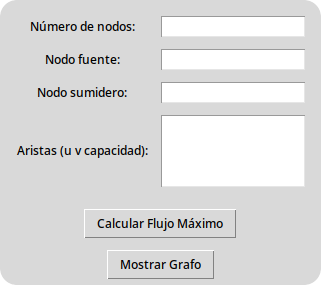
\includegraphics[width=0.5\textwidth]{1.png}
    \caption{Ventana inicial}
    % \label{fig:ventana_inicial}
\end{figure}
Donde ingresaremos lon datos del número de nodos, el nodo fuente, el nodo sumidero y las aristas, que deben ser ingresadas en base a "u", "v" y "capacidad" con un espacio entre cada uno de estos datos y dar un Enter para saltar a la siguiente linea donde ingresaremos la siguiente arista.
Aquí un ejemplo (Datos sacados de la figura  26.5 del libro de ”Introduction to Algorithms por Thomas H. Cormen 2da. Edicion.):

\begin{figure}[h]
    \centering
    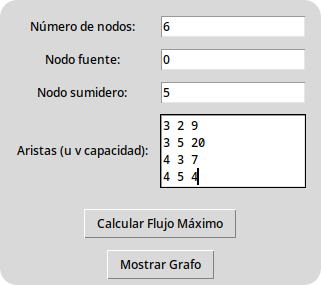
\includegraphics[width=0.5\textwidth]{2.png}
    \caption{Datos de ejemplo}
    % \label{fig:ejemplo}
\end{figure}
\newpage
Una vez ingresados los datos, podemos dar click en "Calcular FLujo Máximo" y obtendremos:

\begin{figure}[H]
    \centering
    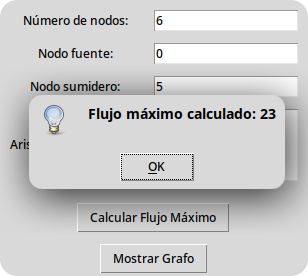
\includegraphics[width=0.5\textwidth]{3.png}
    \caption{Flujo máximo}
    % \label{fig:ejemplo}
\end{figure}
Para ver el grafo generado damos click en "Mostrar Grafo", se habrirá otra ventana con el gráfico deacuerdo a los datos que porporcionamos.

\begin{figure}[h]
    \centering
    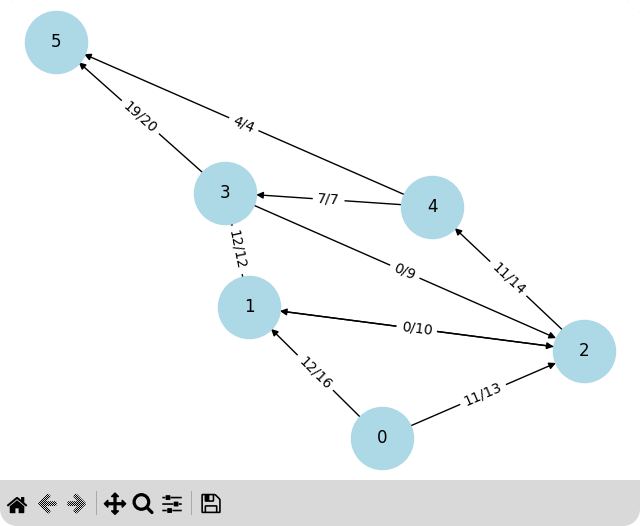
\includegraphics[width=0.5\textwidth]{4.png}
    \caption{Grafo generado}
    % \label{fig:ejemplo}
\end{figure}

En ele grafo se observan los nodos indicados por el usuario además del fujo actual y la capacidad máxima de cada arista.\\
Este programa usa el algoritmo de Edmonds-Karp para calcular la cantidad máxima de flujo que puede pasar desde el nodo fuente al nodo sumidero, respetando las capacidades de los arcos y cumpliendo con la conservación del flujo en los nodos intermedios.

\end{document}

